\subsection{Circuito Pre-amplificador}

\par El circuito pre-amplificador consta de un integrado \textit{TL072} con una configuración de realimentación paralelo-serie, que tiene como fin, amplificar la señal de entrada para ser tratada mediante los filtros siguientes al capacitor de acople $C_{12}$.\\

\par Los filtros tienen como fin disminuir el volumen de las frecuencias bajas o altas a modo de incluir una etapa de procesamiento de señal al proyecto. Esto se logra con los potenciómetros incluidos en la placa, para que el ajuste sea de fácil manejo.\\

\par Por último, se utiliza un divisor resistivo para controlar el volumen del amplificador en conjunto.\\

\begin{figure}[H]
    \centering
    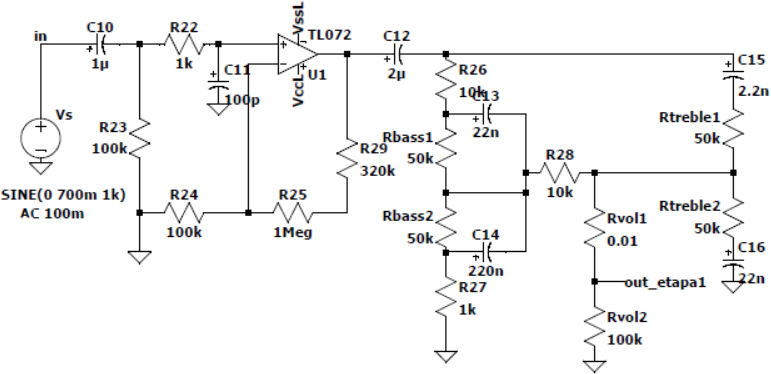
\includegraphics[width=0.75 \textwidth]{img/circuito/pre_amplificador.PNG}
    \caption{Circuito pre-amplificador.}
    \label{fig:ciruito_pre}
\end{figure}

\subsection{Fuente \textit{Switching}}

\par El circuito amplificador se alimenta con 4 tensiones diferentes, las cuales son $+35 \si[per-mode=symbol]{\volt}$, $+15 \si[per-mode=symbol]{\volt}$, $-35 \si[per-mode=symbol]{\volt}$ y $-15V$, para ello se diseñaron dos fuentes switching, una \textit{step down} para bajar de $35 \si[per-mode=symbol]{\volt}$ a $15 \si[per-mode=symbol]{\volt}$ y una \textit{step up} para subir de $-35 \si[per-mode=symbol]{\volt}$ a $-15 \si[per-mode=symbol]{\volt}$.\\

\par A partir de las hojas de datos de los reguladores \textbf{LM2576} y \textbf{LM2577}, en configuraciones indicadas para entregar las alimentaciones correspondientes. Se implementaron los siguientes circuitos tomados de las hojas de datos:\\

\vfill

\clearpage

\begin{figure}[H]
    \centering
    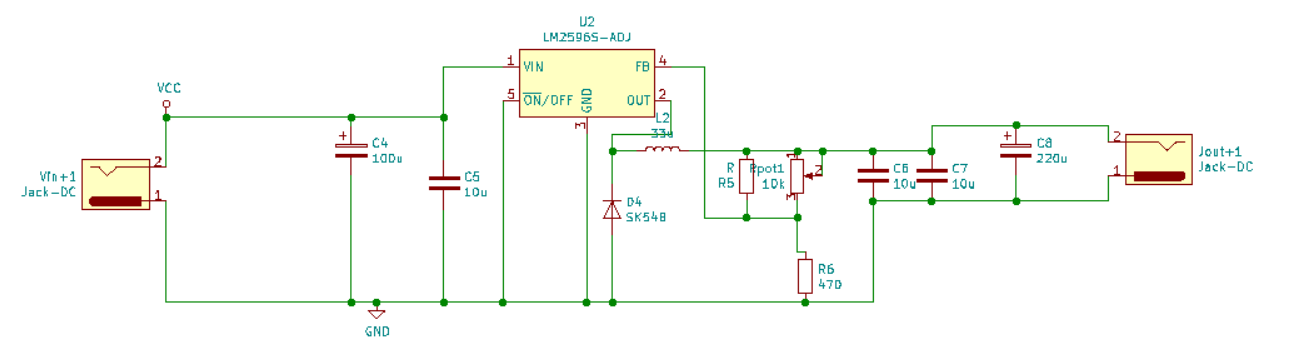
\includegraphics[width=0.95 \textwidth]{img/fuente/fuente_kicad_down.png}
    \caption{Circuito \textit{Step Down}.}
    \label{fig:step_down}
\end{figure}

\begin{figure}[H]
    \centering
    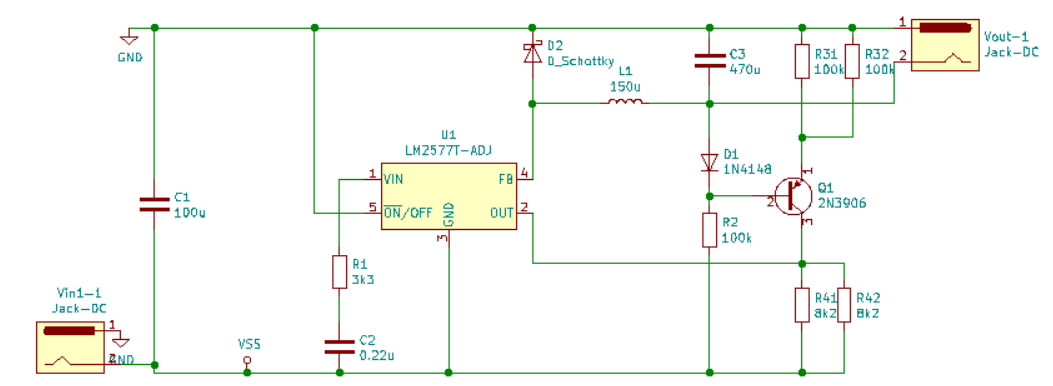
\includegraphics[width=0.95 \textwidth]{img/fuente/fuente_kicad_up.png}
    \caption{Circuito \textit{Step Up}.}
    \label{fig:step_up}
\end{figure}

\par Luego se diseñó el PCB de la fuente \textit{Switching} en \textit{Kicad} a partir de los circuitos mencionados, el resultado se puede observar a continuación:\\


\vfill

\clearpage




\begin{figure}[H]
\centering
\begin{subfigure}{0.5\textwidth}
        \centering
    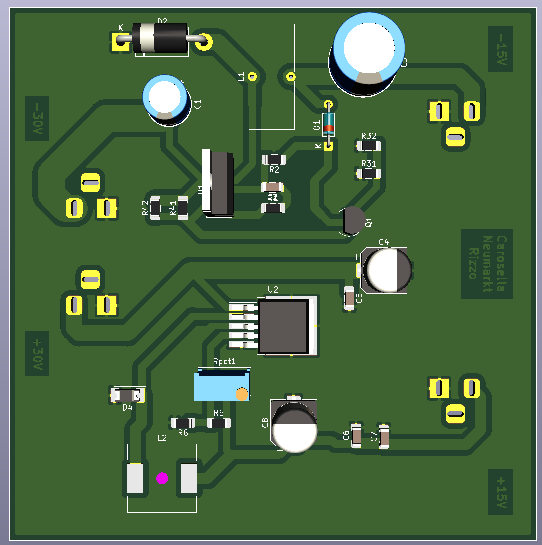
\includegraphics[width = 0.95 \textwidth]{img/fuente/fuente_switching_3D.PNG}
        \caption{Vista superior.}
        \label{fig::fuente_3D_T}
\end{subfigure}%
\begin{subfigure}{0.5\textwidth}
        \centering
    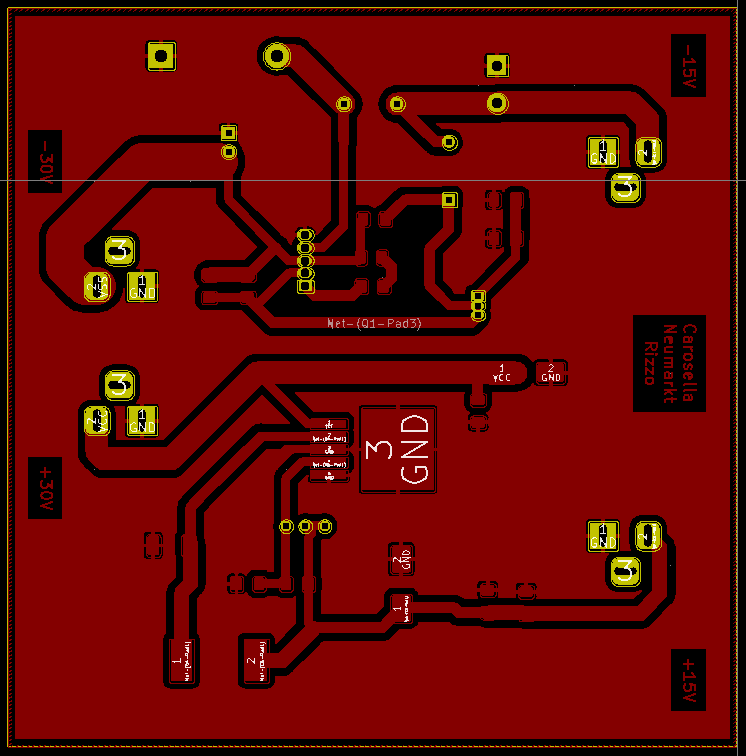
\includegraphics[width = 0.95 \textwidth]{img/fuente/fuente_switching.PNG}
        \caption{Vista inferior.}
        \label{fig::fuente_3D_B}
\end{subfigure}
\caption{Vista 3D del PCB de la fuente switching interna.}
\label{fig:fuente_3D}
\end{figure}



\subsection{Circuito amplificador}


\par A continuación, se muestran el esquemático del circuito implementado en \textit{Kicad}. En primer lugar, en la figura \figref{fig::ampli_kicad} muestra el amplificador principal clase G diseñado junto con el circuito de pre-amplificador. Luego se prosiguió por realizar el diseño del PCB. Para ello se aplicó un plano de masa en la capa superior de la placa. Por otro lado se utilizaron pistan anchas y cortas, de un espesor de $60 \si[per-mode=symbol]{\mils}$ a $118 \si[per-mode=symbol]{\mils}$ y separaciones entre pistas mayores a $12 \si[per-mode=symbol]{\mils}$. Seguidamente se muestran imágenes del PCB para el amplificador clase G a implementar.\\


\vfill

\clearpage



\begin{figure}[H]
        \centering
        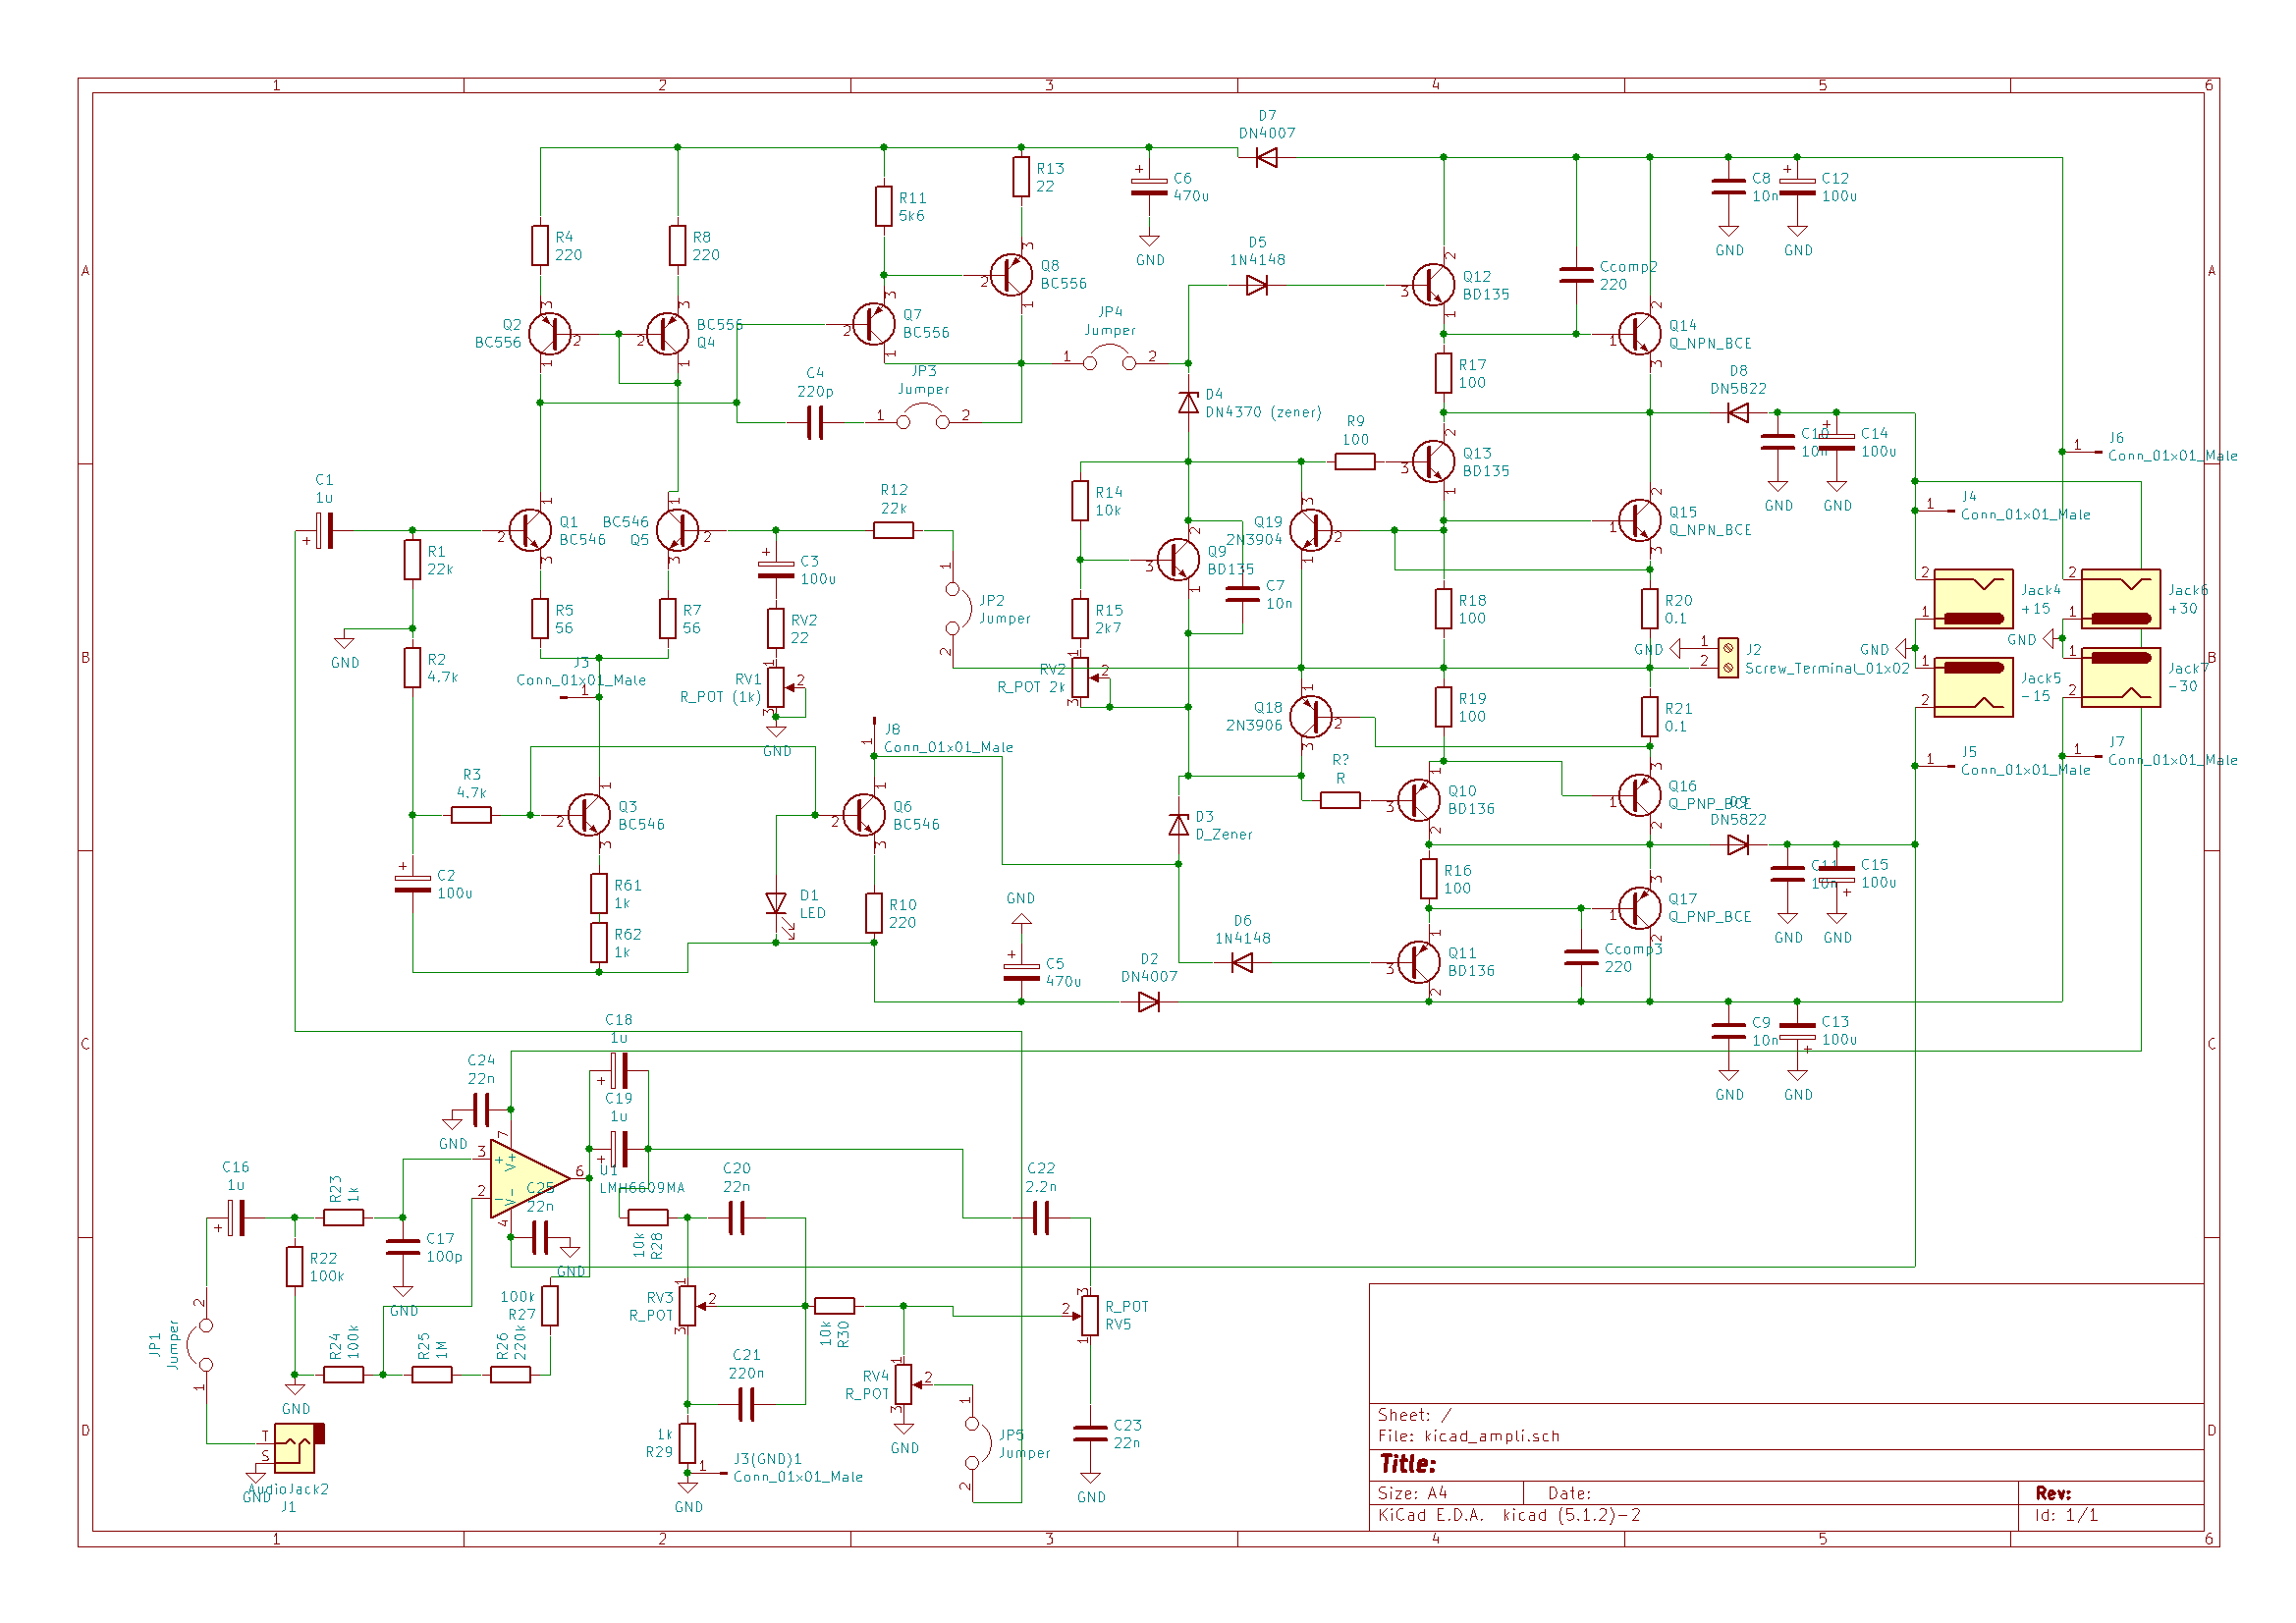
\includegraphics[height=0.8 \textwidth, angle=90]{img/circuito/kicad.png}
        \caption{Esquemático de amplificador con clase G.}
        \label{fig::ampli_kicad}
\end{figure}

\begin{figure}[H]
        \centering
        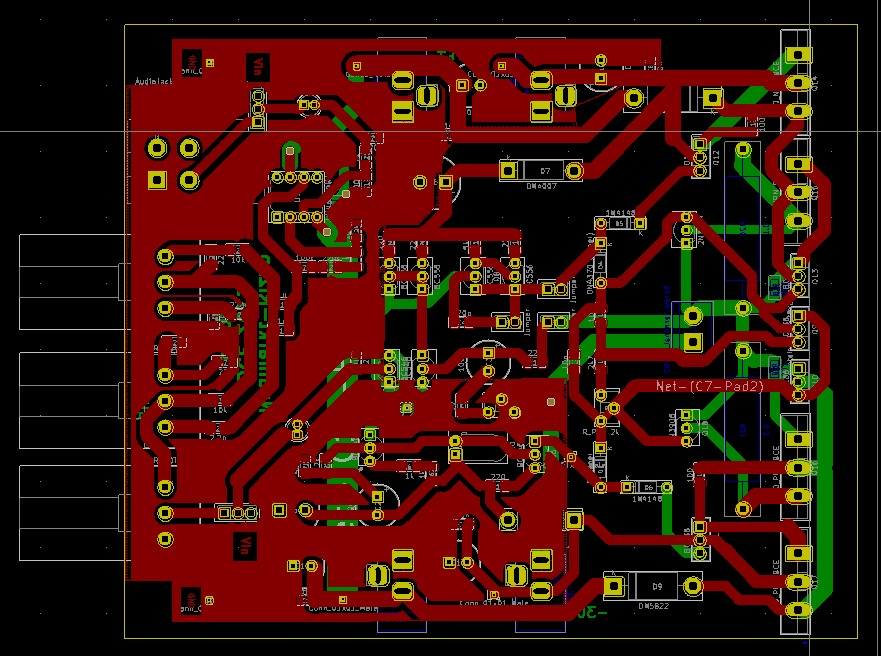
\includegraphics[width=0.65 \textwidth]{img/circuito/PCB1.jpeg}
        \caption{PCB del amplificador.}
        \label{fig::amp_PCB1}
\end{figure}


\begin{figure}[H]
\centering
\begin{subfigure}{0.5\textwidth}
        \centering
        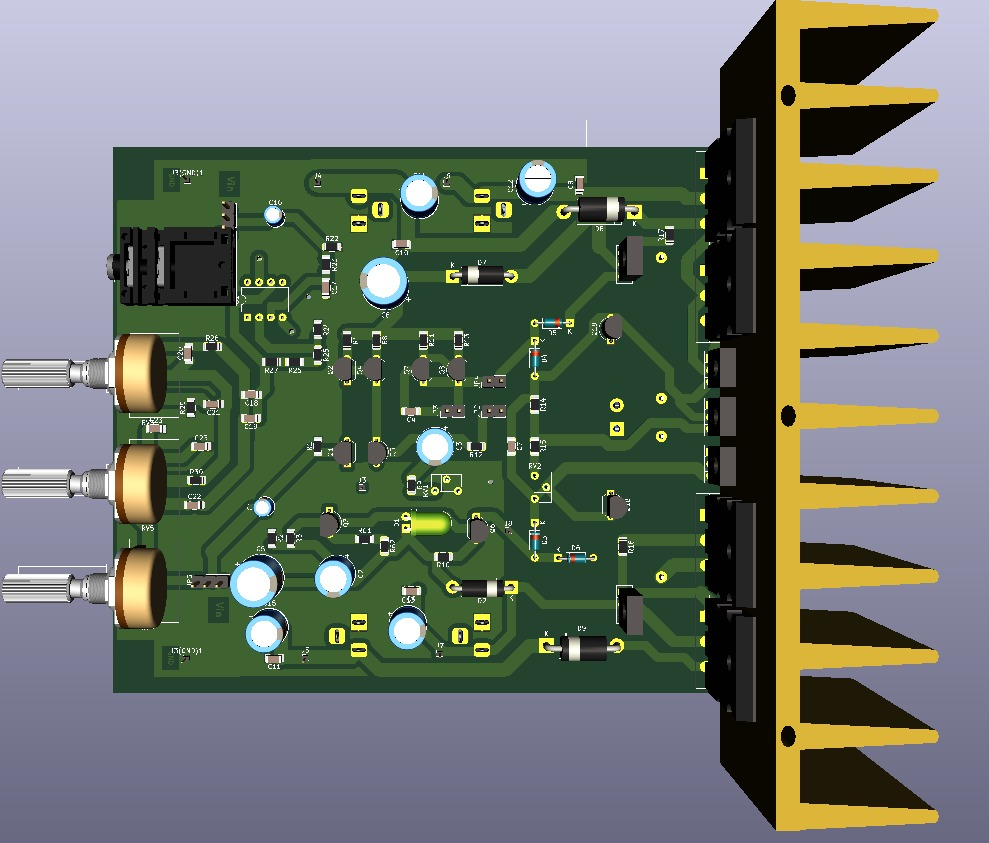
\includegraphics[width = 0.95 \textwidth]{img/circuito/PCB_3D_Top.jpeg}
        \caption{Vista superior.}
        \label{fig::PCB_3D_T}
\end{subfigure}%
\begin{subfigure}{0.5\textwidth}
        \centering
        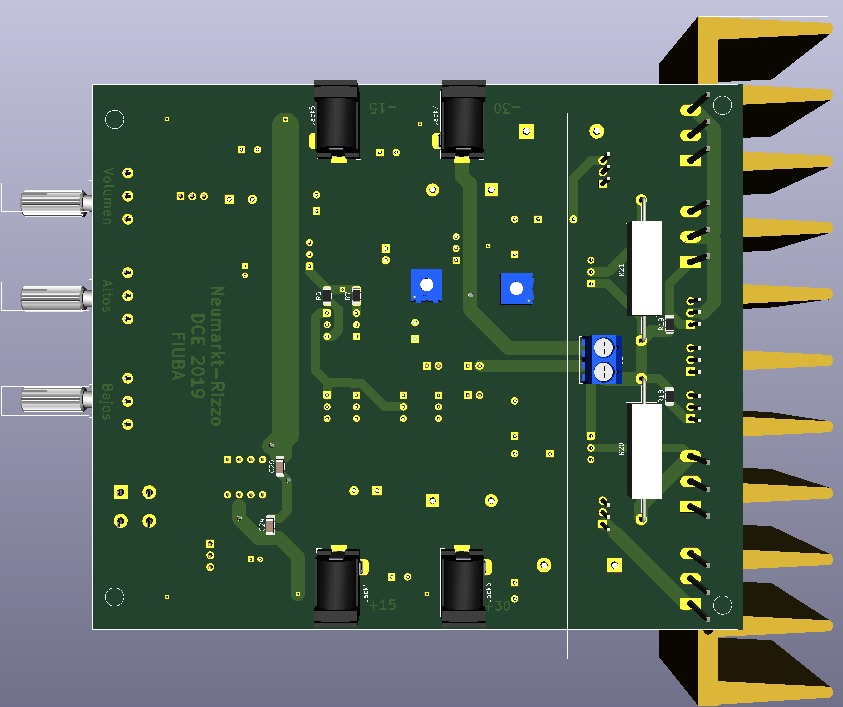
\includegraphics[width = 0.95 \textwidth]{img/circuito/PCB_3D_Bot.jpeg}
        \caption{Vista inferior.}
        \label{fig::PCB_3D_B}
\end{subfigure}
\caption{Vista 3D del PCB del amplificador.}
\label{fig:PCB_3D}
\end{figure}

